\begin{frame}{Modelo Discriminador}
    

    El modelo SRGAN (Super Resolution Generative Adversarial Network) fue
    propuesto en 2016 por un grupo de investigadores de la empresa Twitter.
    La principal innovación de este modelo es su función de pérdida, llamada
    función de pérdida perceptual, que permite mejorar el realismo de la imagen de
    salida.

        
    \begin{figure}[H]
        \begin{center}
          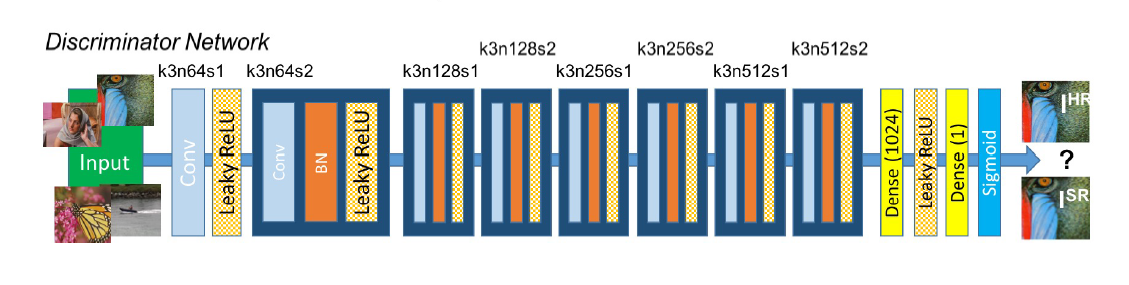
\includegraphics[scale = 0.5]{Imp_discriminador.png}
          \caption{Modelo de entrenamiento del discriminador}
          \label{Alexis3}
        \end{center}
    \end{figure}
     

\end{frame}

\begin{frame}{Modelo Discriminador}
    

    El modelo SRGAN (Super Resolution Generative Adversarial Network) fue
    propuesto en 2016 por un grupo de investigadores de la empresa Twitter.
    La principal innovación de este modelo es su función de pérdida, llamada
    función de pérdida perceptual, que permite mejorar el realismo de la imagen de
    salida.

        
    \begin{figure}[H]
        \begin{center}
          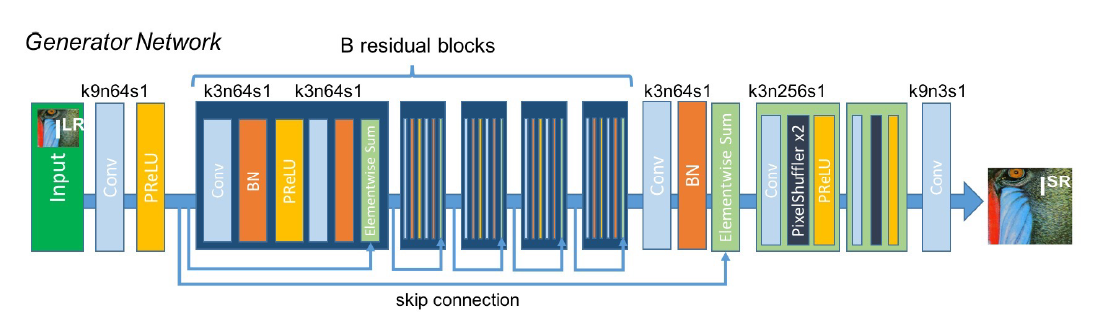
\includegraphics[scale = 0.5]{Imp_generador.png}
          \caption{Modelo de entrenamiento del generador}
          \label{Alexis4}
        \end{center}
    \end{figure}
     

\end{frame}



\begin{frame}{Modelo Discriminador}
    

        
    \begin{figure}[H]
        \begin{center}
          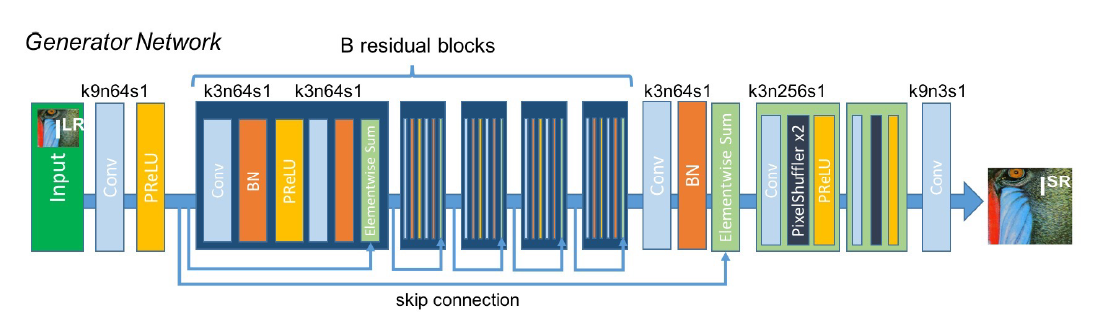
\includegraphics[scale = 0.5]{Imp_generador.png}
          \caption{Modelo de entrenamiento del generador}
          \label{Alexis5}
        \end{center}
    \end{figure}
     

\end{frame}


\begin{frame}{Modelos Generadores obtenidos}
    
    \begin{figure}[H]
        \begin{center}
          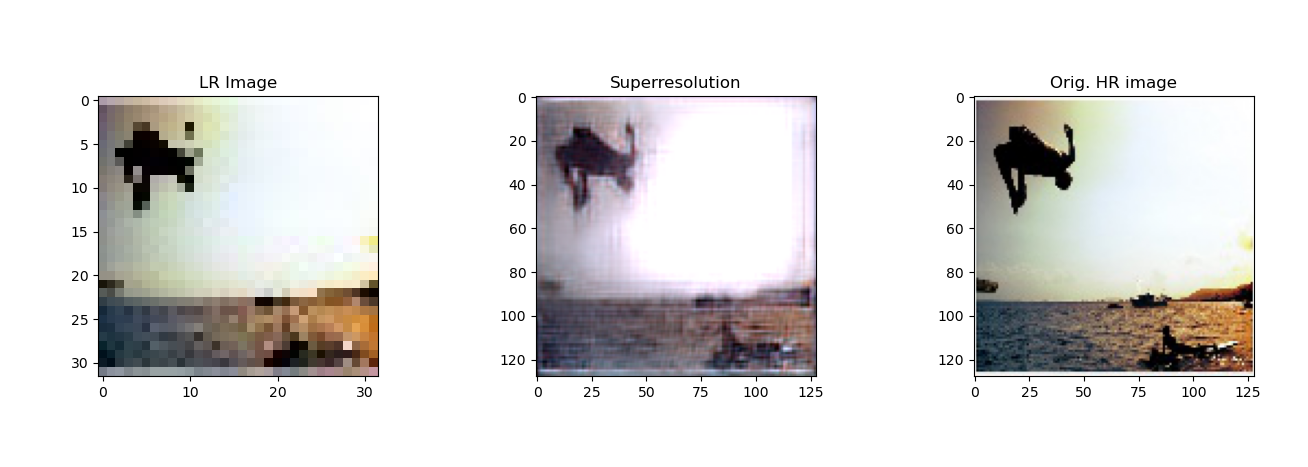
\includegraphics[scale = 0.5]{13im_200E.png}
          \caption{Modelo de entrenamiento del generador}
          \label{Alexis6}
        \end{center}
    \end{figure}
    
\end{frame}

\begin{frame}{Modelos Generadores obtenidos}
    
    \begin{figure}[H]
        \begin{center}
          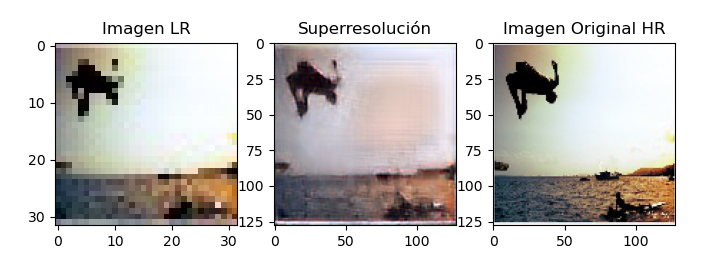
\includegraphics[scale = 0.5]{50im_400E.png}
          \caption{Modelo entrenado con 50 imágenes y 400 épocas}
          \label{Alexis7}
        \end{center}
    \end{figure}
     
\end{frame}


\begin{frame}{Modelos Generadores obtenidos}
    
    \begin{figure}[H]
        \begin{center}
          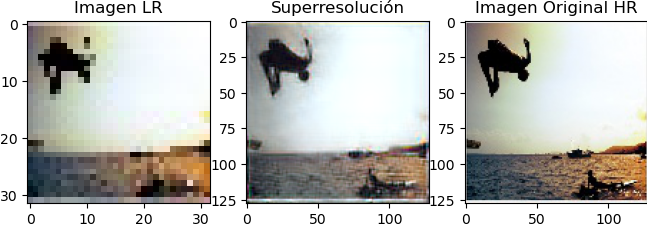
\includegraphics[scale = 0.5]{1000im_5E_Reentrenado.png}
          \caption{Modelo reentrenado 1000 imágenes, 5 épocas}
          \label{Alexis8}
        \end{center}
    \end{figure}
     
\end{frame}